\documentclass[letterpaper]{article}

\usepackage{graphicx}
\usepackage{listings}
\usepackage{url}
\lstset{language=C}

\newcommand{\code}[1]{\texttt{#1}}

\title{SkyeFS: A FUSE Filesystem Providing Distributed Directories using Giga+
and PVFS}
\author{Anthony Chivetta \url{<anthony@chivetta.org>}\\Swapnil Patil \& Garth
Gibson}
\date{DRAFT --- \today}

\begin{document}

\maketitle

\section{Overview}
PVFS, the Parallel Virtual File System, stores all metadata for a particular
directory on a single metadata server.  As a result, PVFS metadata performance
on large or highly trafficked directories is poor. Giga+ is a scheme for
distributing the metadata for a directory across a set of servers.  SkyeFS
implements the Giga+ algorithms on top of an unmodified PVFS file system.

SkyeFS consists of a client (\code{skye\_\-client}) which functions as the FUSE filesystem
and a server (\code{skye\_\-server}) which provides synchronization for metadata
operations and controls directory placement and splitting.  

Giga+ operates by splitting a directory into multiple partitions, which may or
may not be on the same server, but act as distinct metadata stores.  Because in
PVFS each directory stores all its metadata together on a single server, we
represent each Giga+ partition as a distinct PVFS directory.  A SkyeFS server
running on each PVFS metadata server (MDS) provides the synchronization and
coordination for the partitions on the local PVFS MDS. 

This paper presents the design and implementation decisions behind SkyeFS and
their rational.  When appropriate, we also indicate places where future work is
needed.  It is our hope that the design decisions made here may help inform
future implementations of Giga+ or other systems on top of PVFS.

\section{Implementation Overview}
We choose to implement Giga+ on top of PVFS instead of modifying PVFS itself in
order to keep the implementation clean and simple.  FUSE provides an easy option
for implementing the client side of the system due to the ease of writing a FUSE
file system driver.  Additionally, the pvfs2\-fuse application distributed with
the PVFS source provides an example of how to implement FUSE operations in PVFS.

In PVFS, each object, both directories and files, are assigned a PVFS metadata
handle.  Each MDS is assigned a range of handles for which it is responsible.
In the case of directories, the MDS responsible for a given directory's handle
will contain all the directory entries for that directory.  Therefore, we can
achieve partitioning of files between servers by ensuring that the directory
entries fall in directories whose handles are owned by different MDSs.  

\subsection{Physical Layout}
Through testing and reading of the PVFS source code, we determined that moving
a file between directories, either on the same or different MDS, moves only
the directory entry and not the entire file.  Therefore, we store each Giga+
partition in a distinct PVFS directory instead of putting all Giga+ partitions
in one directory per server.  We believe that the cost of having to sometimes
split onto a local server is outweighed by the benefit of minimizing total
directory size.

Upon creation of a logical directory, ``foo'', we create a PVFS directory of
the same name.  Inside that PVFS directory, we create a PVFS directory for the
first Giga+ partition called ``p00000''.  The `p' signifies that this is an
active partition, while the ``00000'' provides the partition number.  When
this partition splits, the directory ``p00001'' will be created adjacent to it
to store the files in the new partition.  This gives rise to the invariant
that every other directory in a PVFS path must be a partition of a logical
directory.  For example, the path ``/p00005/foo/p00001/bar'' is a valid path,
but ``/p00003/foo/bar'' is not.

The location for a new PVFS directory is determined by the PVFS client using
round robin assignment, however there is no way to influence this
decision.  To avoid requiring a modified PVFS client, we have implemented an
initial naive solution to controlling the placement by simply removing and
recreating a directory until it is placed by the PVFS client on the correct
server.  Future improvements to the code could improve the efficiency of
this code by caching the created directories, either in a per-directory or
per-filesystem manor.  

In the per-directory case, when an unneeded directory is created it is renamed
from ``p$n$'' to ``u$m$'' where $m$ is the first partition that does not yet
exist but will be placed on that directory's MDS.  Prior to creating a
directory for partition $n$, the system will check for the existence of
``u$n$'' and rename it to ``p$n$'' if found.

In the per-filesystem case a global scratch directory is maintained in which
unused directories are placed.  Prior to creation of a new partition, this
directory is searched for a directory on the correct server.  This has the
advantage of leaving fewer unused directories on the file system but in systems
with a high rate of splits could create a directory with a high rate of
concurrent activity.

\subsection{Path Translation}
\begin{figure}
\begin{center}
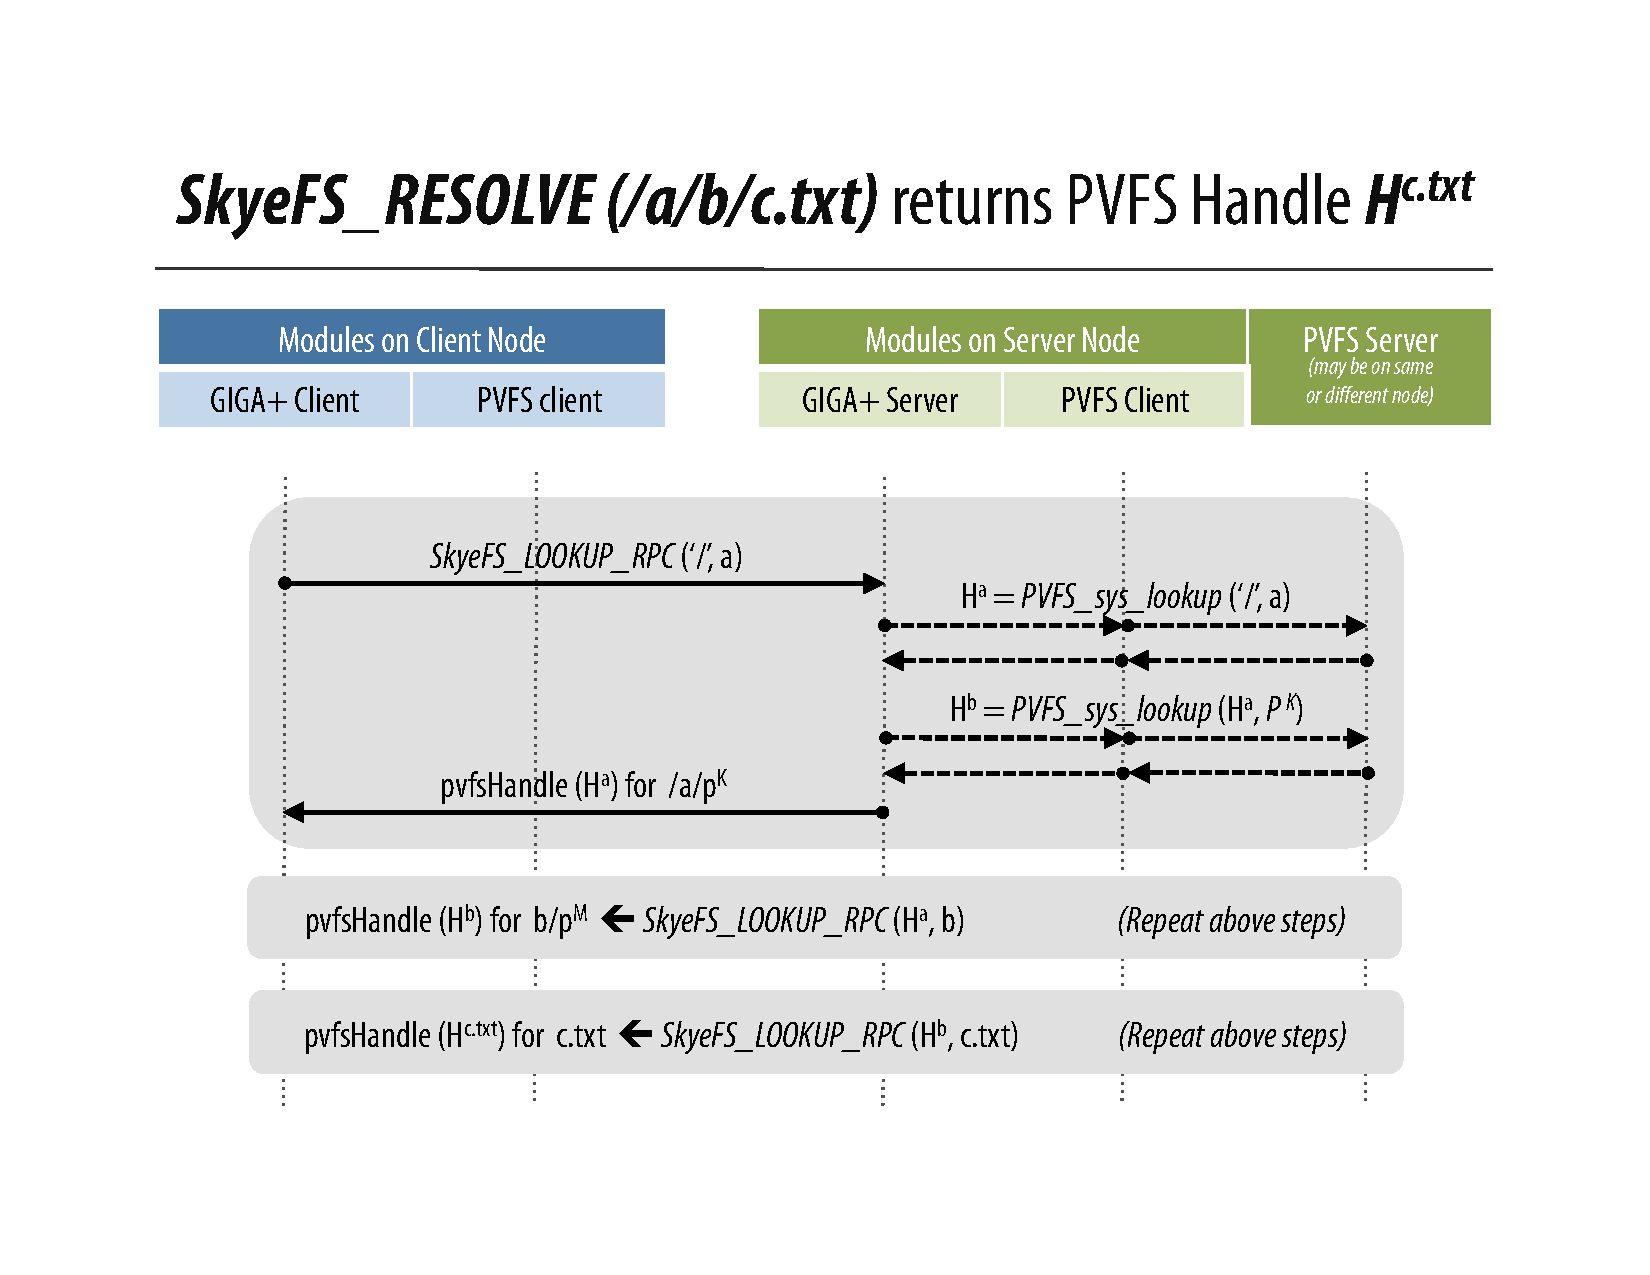
\includegraphics[scale=0.4]{figure-resolve}
\end{center}
\caption{SkyeFS Name Resolution}
\end{figure}
Given this layout, we must determine how clients are to translate logical path
names to their respective PVFS objects.  The PVFS system interface uses PVFS
handles to specify operands for most filesystem operations.  PVFS provides
\code{PVFS\_\-sys\_\-lookup(path)} and
\code{PVFS\_\-sys\_\-ref\_\-lookup(parent handle, name)} to translate either
an absolute or relative path to a PVFS handle.  We implement our own
\code{lookup(parent handle, name)} that resolves one logical path component.
For example, calling \code{lookup(NULL, ``foo'')} would return the PVFS handle
of ``/p00004/foo'' if ``foo'' was stored in the fifth partition of the
filesystem root.  If we let that handle be $h$, then calling \code{lookup($h$,
``bar'')} would return the PVFS handle of ``/p00004/foo/p00002/bar'' if
``bar'' is in the third partition of ``foo''.  In this manor, any logical path
can be resolved to its PVFS handle in a manor opaque to the caller.  For
convenience, we provide a \code{resolve(path)} that iterates through the
provided path calling \code{lookup()} at each step.

PVFS metadata handles do not change when their objects are moved between
directories.  Therefore, the handle returned by lookup is guaranteed to continue
to be a valid reference to the object for the duration of the object's
existence.  This is true even if the partition holding an object splits or the
logical directory is moved elsewhere in the directory tree.  As a result, we can
safely hold a PVFS handle for the duration of a FUSE operation or between calls
to \code{open()} and \code{close()} without having to check its validity.

\subsection{Client/Server Architecture}
\begin{figure}
\begin{center}
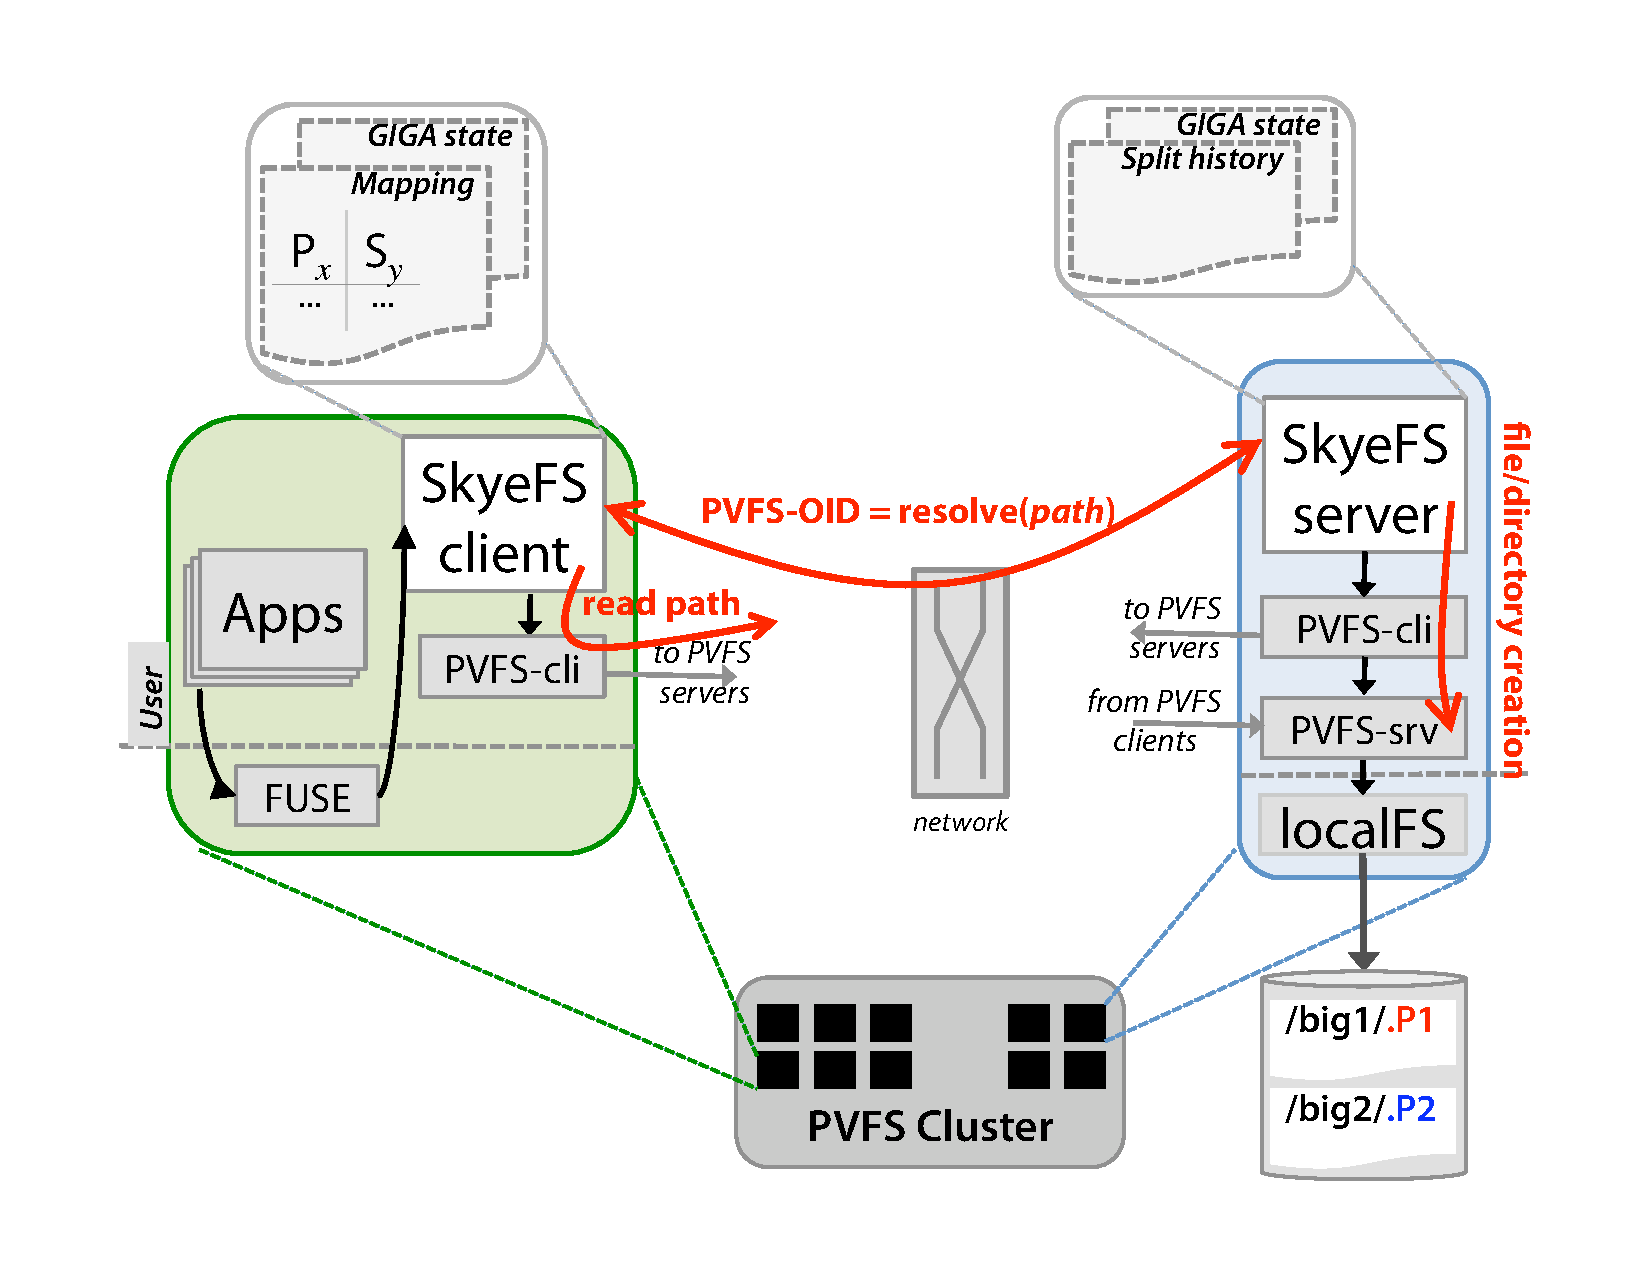
\includegraphics[scale=0.4]{figure-architecture}
\end{center}
\caption{SkyeFS Architecture Diagram}
\end{figure}
\code{lookup()} needs to be able to determine the partition in which an object
should live before it can issue the appropriate \code{PVFS\_\-sys\_\-lookup()}
call to determine an object's handle.  For this to be done quickly, and with a
minimum of PVFS calls, we use a \code{skye\_\-server} process to maintain in
RAM a bitmap representing the state of a directory.  The \code{skye\_\-server}
process runs on each PVFS MDS and is responsible for coordinating access to
the partitions living on that MDS.  It implements a handful for ONC RPC calls,
including \code{lookup()}, that are used by the \code{skye\_\-client} to
operate in or on the partitions handled by that server.  In the case of
lookup(), the server consults its mapping and issues a PVFS lookup for a
rewritten path including the partition of the object.

The mapping between hash values and partitions/servers is determined by the
values in a \code{struct giga\_\-mapping}.  Both the client and server
maintain read-through caches for these structures.  In the event of a cache
miss, the system will interrogate PVFS for appropriate initial data.

For performance and load-balance considerations, locality between the
\code{skye\_\-server} process and the PVFS server to which it is making
requests is maintained whenever possible.  Each RPC response includes an error
code.  Upon receiving a RPC request, the server will determine if it owns the
partition on which the request will operate.  If not, the server will return
EAGAIN as the error code and provide the client with a copy of its own mapping
for the directory.  Upon receiving this error code, the client will read the
server provided mapping and merge that information with its local version.
The client will then reattempt the RPC call to a new \code{skye\_\-server} as
per the updated mapping.  This ensures both that locality as maintained and
that the client's cached mapping will tend toward reality.

The \code{skye\_\-server} process is also used to prevent a variety of race conditions.
By forwarding all operations that operate on a file path or name, as opposed to
only a PVFS handle, to the \code{skye\_\-server} we ensure that splitting does not
interfere with successful execution of thees commands.  For example, during a
create operation, the \code{skye\_\-server} thread issuing the create will lock a data
structure for the directory so that the partition is prevented from splitting
until the create can finish.  However, while simply forwarding all the work of
potentially conflicting operations to a \code{skye\_\-server} would be an easy solution to
concurrency problems, we attempt to offload the absolute minimum amount of work
to the \code{skye\_\-server} to ensure that it does not become a bottleneck.

\subsection{Metadata Persistence}
Closely related to the issue of physical layout is that of persisting SkyeFS
metadata.  This includes the Giga+ mapping (the bitmap and zeroth server), the
server list at the time of directory creation and the state of any splitting
directories.  To make the system as fault tolerant as possible, we avoid
explicitly storing any of this metadata and instead interrogate the state of a
directory in PVFS to determine these values.

Rather than building into SkyeFS our own mechanism for maintenance of server
lists we simply ask PVFS for the current server list on start up.  Tests indicate
that PVFS will always return this in the same order.  In the event of a server
addition the new servers are simply added to the end of the list.  As PVFS does
not support the removal of servers, we do not need to provide support for that
functionality.  Therefore, to determine the server list at the time of a
directory creation we only need to know the number of servers that existed when
the directory was created.

When the server's read-through cache suffers a cache miss it must populate a new
\code{struct skye\_\-directory} with the necessary information.  It determines
the zeroth server by asking PVFS for the MDS responsible for the directory's
PVFS handle.  It then performs a \code{readdir()} on the directory to find all
existing partitions (folders with the `p' prefix).  This also will reveal any
currently splitting partitions (folders with the `s' prefix).  If the server
determines that it is responsible for completing an unfinished split it will
enqueue the partition for completion by the split thread.\footnote{This is
currently unimplemented.} It will then read an extended attribute from the
directory that indicates the number of servers which existed when the
directory was created.\footnote{This is currently unimplemented.}  This
extended attribute is only ever written once, at the time the directory is
created, so there is no risk of inconsistency being introduced by directory
operations.  All the other values similarly do not face any inconsistency
risks as they are simply functions of the physical layout of the directory.

On the client side we use a significantly simplified version of the cache
population procedure to avoid hitting the PVFS servers.  When the read-through
cache suffers a miss it will simply create a new object with a bitmap consisting
of only the zeroth partition, a server list of length one and the zeroth server
set to the owner of the directory's handle.  The merging semantics of Giga+
mappings ensure that as the client receives updated mappings from the servers
this initial mapping will tend toward accurate.

Populating the initial mapping in this way causes the \code{lookup()} code to always
start with the zeroth server in the cache-cold state.  While this ensures that
some progress towards finding the correct server is always made, it has the
potential to cause unbalanced load on servers which act as the zeroth server for
popular directories.  One potential solution to this problem is to provide
bootstrapping hints to clients during the iterative \code{lookup()} process.
When a client performs a {lookup()} and the server detects that the object is
a directory the server should also return any cached bitmap it may have for
that directory to the client to populate its cache.  This would improve the
performance of cache-cold and cache-warm lookups by reducing the number of
servers a client must contact before it reaches the correct server. 

This persistence scheme results in a system that can halt at almost any time
without leaving the system in an inconsistent state.

\section{Filesystem Operations}
\subsection{Splitting, and create()}
\begin{figure}
\begin{center}
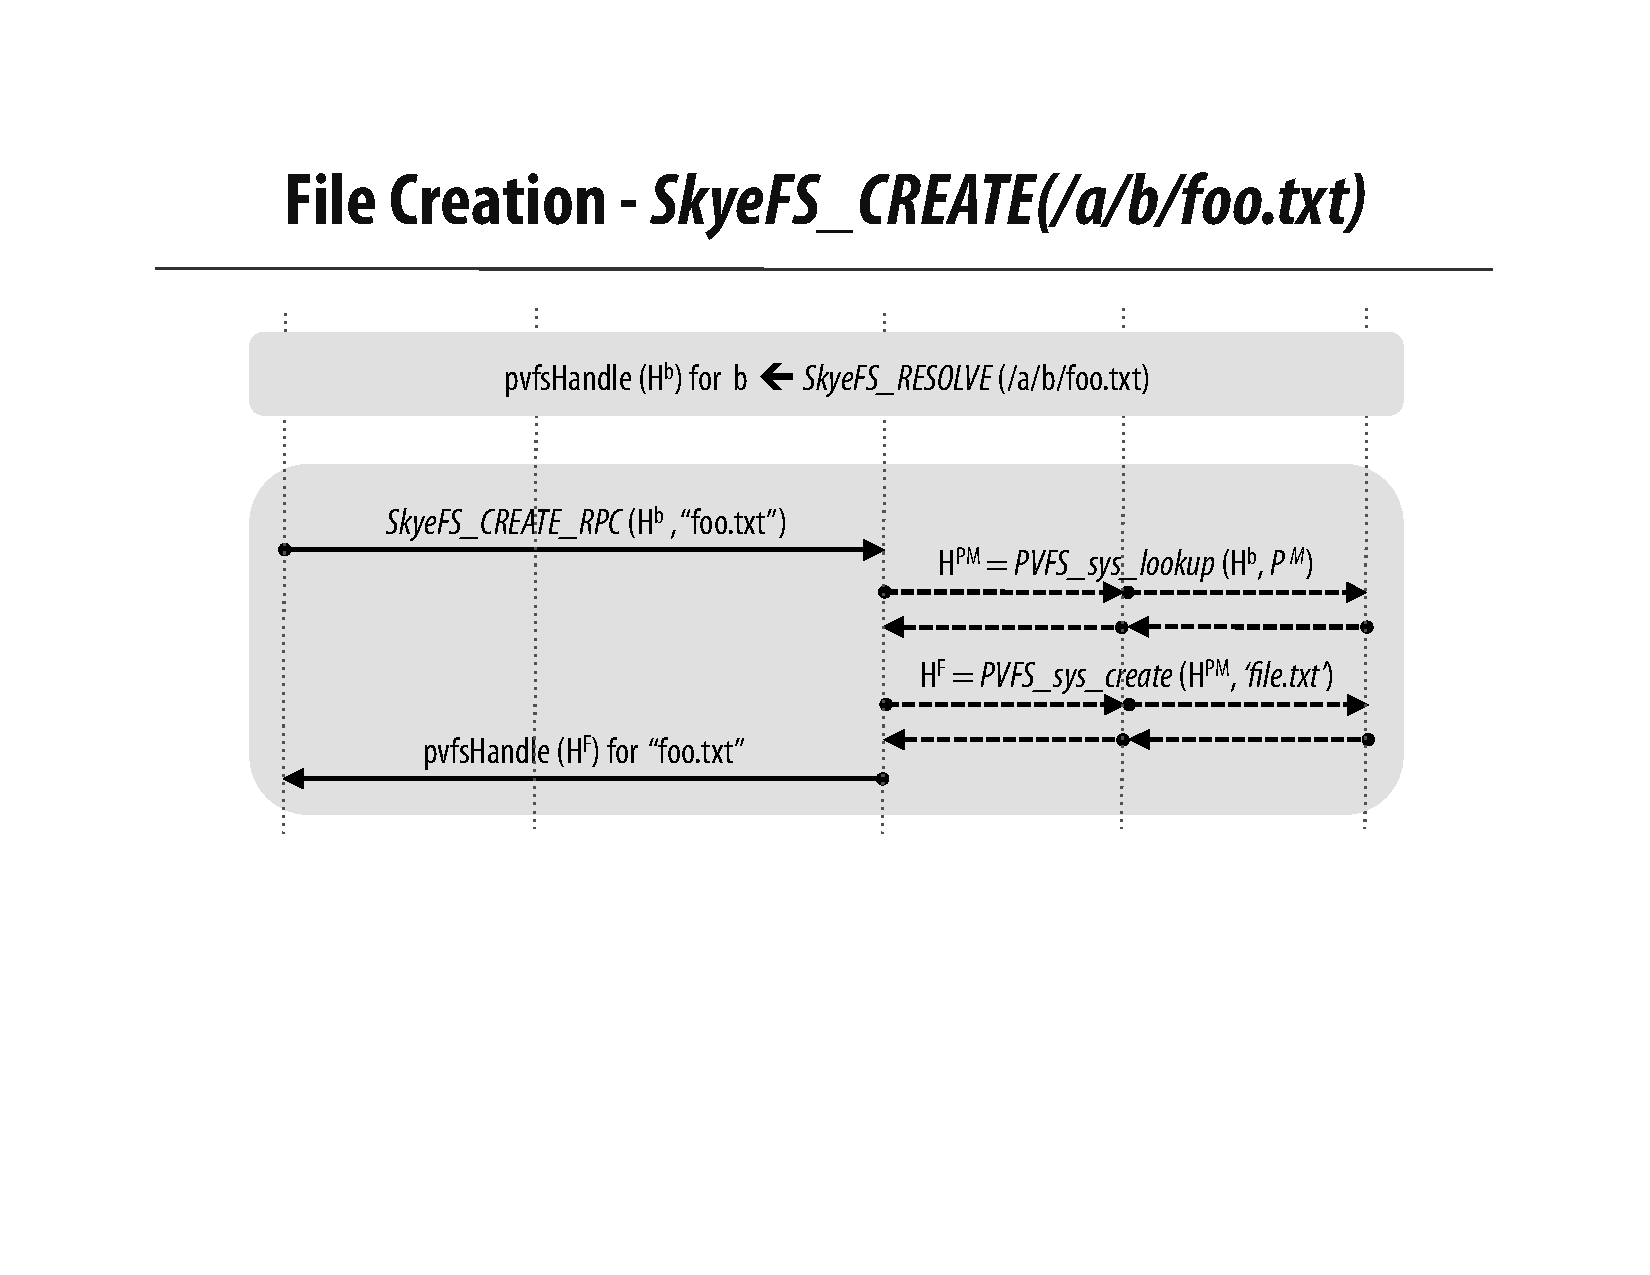
\includegraphics[scale=0.4]{figure-create}
\end{center}
\caption{SkyeFS Create Procedure}
\end{figure}
The \code{create()} RPC is used by \code{skye\_\-client} to create files in a given
directory.  Just like with \code{lookup()} only the server that owns the correct
partition for a file will service a \code{create()} call.  Quite simply, the
\code{create()} RPC calls \code{PVF\_\-sys\_\-create()} with the appropriate
parent handle.  The complex part is handling splitting during and after a
\code{create()}.

Splitting of partitions is a critical and potentially tricky part of the Giga+
algorithm.  In PVFS we are able to achieve a high degree of concurrency in the
face of splitting thanks to the stability of PVFS file handles and the rename
semantics.

Each logical directory is represented by a \code{struct skye\_\-directory} on
the server.  This structure is defined approximately as follows:

\begin{lstlisting}
struct skye_directory {
    giga_mapping mapping;
    int reference_count;
    PVFS_object_ref PVFS_handle;
    int splitting_index;
    pthread_rwlock_t rwlock;
    UT_hash_handle hashtable_handle;
};
\end{lstlisting}

During normal operation, when no splits are happening,
\code{splitting\_\-index} has the value of -1.  When an operation needs to
access the directory, it acquires a read lock on the read-write lock for the
duration of the operation.  By holding the read-write lock, the operation can
be assured that no partition will begin to split until the lock is released.

At the end of the \code{create()} call, a \code{stat()} operation is performed
on the partition and the number of directory entries in the partition is
compared to the system's split threshold.  If the current directory size is
greater, the PVFS handle of the parent and the partition number are stored at
the end of a queue of partitions to split.  The \code{create()} call then
returns as normal.

Each \code{skye\_\-server} has a dedicated splitter thread.  This thread waits on a
condition variable associated with the split queue.  When an operation adds a
entry to the queue it signals on the condition variable to wake up the splitting
thread.  The splitting thread iterates through the queue and splits all
specified partitions which are found to still be over the splitting threshold.

To split a partition, the splitting thread first acquires a write lock in the
directory.  This ensures that all operations currently outstanding on the
directory are finished before the lock is acquired and that no new operations
may begin.  The splitting thread then creates the destination partition using a
`s' prefix instead of a `p' prefix in order to indicate, in the event of system
failures, that a partition is still in the process of splitting.\footnote{This
is currently unimplemented.}  It also sets the \code{splitting\_\-index} field
to be the index of the splitting partition.  The splitting thread then unlocks
the directory to allow operations to continue.

The splitting thread performs a \code{readdir()} operation on the partition to be
split.  For each entry, it hashes the name to determine if the object is to be
moved to the new partition and then executes the move, using the PVFS
\code{rename()} operation, if necessary.

While this is happening, any thread that accesses the directory will notice that
\code{splitting\_\-index} is not set to -1.  For creation operations, the
correct post-split partition will automatically be used ensuring that the new
object will end up in the correct partition.  For access operations such as
lookup(), first the old directory will be checked and if the object is not
found there the new directory will be checked.  The PVFS rename() operation
ensures that a renamed file is always visible in at least one of the source or
destination directories.  Therefore, this technique is guaranteed to always
find the object if it exists.  The read-write lock is necessary for this technique to
work because the operation must know for certain that the partition it
accessed did not split during the operation.  If the operation simply checked
the bitmap at the end of the operation it would be able to retry but this
could lead to starvation, or at least many operations being forced to retry or
correct inconsistent data.

Upon completion of the split, the splitting thread reacquires a writer lock on
the directory.  It renames the directory to begin with the prefix `p' instead of
`s' and then sends a \code{bucket\_\-add()} RPC to the server responsible for the new
partition.  Upon positive reply the server updates its copy of the bitmap, sets
the \code{splitting\_\-index} back to -1 and unlocks the rwlock.  In the event that
a positive reply is not provided by the destination server, the source server
may still provide service to that partition by leaving the
\code{splitting\_\-index} set and not updating the bitmap.\footnote{This is
currently unimplemented.}  This will force operations to continue to check
both directories.  The splitting thread now sleeps and retries the
\code{bucket\_\-add()} RPC until it succeeds.  In this failure case, we
intentionally avoid splitting new partitions to ensure that we don't create
many new ``orphaned partitions''.

We use a separate splitting thread for this operation to ensure that splittings
are entirely asynchronous.  As a result, file system operations are able to
happen even while a partition is being split.  This can result in significantly
improved performance over implementations that must block during a split.  The
separate split thread also ensures that operations threads can do the bare
minimum amount of work during the create operation and leave splitting for
later.  We use only one splitting thread because we don't want to split two
partitions at a time due to the potential for resource contention with other
operations at the PVFS server.  In addition, this allows us to simplify our data
structures for each directory significantly because we only have to note one
splitting partition at a time.

\subsection{mkdir()}
Our directory creation code extends \code{create()}'s locking and splitting
functionality to handle a few directory creation issues.  Instead of using
\code{PVFS\_\-sys\_\-create()} to create a file, the \code{PVFS\_\-sys\_\-mkdir()} call is
used to create the logical directory.  The server on which that directory was
created is determined by the handle of the new directory.  A new sub directory
call``p00000'' is created on the same server as the zeroth partition of the
directory.  This ensures that the zeroth server can be determined by looking
at the logical directory's handle in addition to the zeroth partition's handle.
The handle of the newly created directory is then passed back to the client.

When the client first attempts to access the new directory it will contact the
zeroth server for that directory as part of the cache population process.  That
server will also undergo the cache population process and find that it owns the
zeroth partition of that directory.  From the perspective of the destination
directory, the creation of a new directory is indistinguishable from the first
(cache cold) access of an existing, empty directory.

Should the server doing directory creation fail between the creation of the
logical directory and the first partition an inconsistent state will be
left.\footnote{This is currently unimplemented}  In the event that such a
directory is encountered by the server it can simply delete the directory to
return to a consistent state.  This check could be implemented as part of a
fsck process.

\subsection{remove()}
The remove operation for a file is a relatively simple operation.  We use the
same logic as the \code{lookup()} operation for finding a file in a partition
and then simply issue a \code{PVFS\_\-sys\_\-remove()} for that object.

Directories are another story.  The remove operation on a directory must fail if
there exists any files in the directory, otherwise the directory must be
removed.  This means that we need to be able to remove the directory
atomically from the perspective of the user and ensure that any concurrent
create() operations either fail or cause the remove() to fail.

To coordinate removal of a directory, we implement a server to server RPC call
called \code{bucket\_\-remove()}.  The client attempting to remove a directory will send a
\code{remove()} RPC to the server holding the directory entry for the directory.  The
server will then issue a \code{bucket\_\-remove()} RPC for each bucket in descending order
(i.e. the highest numbered bucket first).  

When a server receives this call it will attempt to remove the specified
partition by issuing a \code{PVFS\_\-sys\_\-remove()} for the directory.  If the operation
succeeds then the partition will be removed from the owner's bitmap and the
owner will return a positive response to the caller.  The caller will also
remove the partition from its bitmap and then issue the next
\code{bucket\_\-remove()}.

If the \code{PVFS\_\-sys\_\-remove()} fails (for any reason other than \code{ENOENT}) the partition
will remain in the bitmap and a negative response will be returned to the
server.  The coordinating server will then halt the operation and return an
error to the client.  In this case care must be taken to ensure that the system
is left in a consistent state.  By removing the partitions in descending order
we ensure that we always remove the parent of a split before its child.
Therefore, each intermediate bitmap (produced between
\code{bucket\_\-remove()} calls) is
a valid bitmap in itself.

We also need some mechanism to update client bitmaps to remove the now missing
partitions.  The merge operation performed by the client does a logical
OR of the old and new bitmaps making it unable to handle a removal.  Instead, we
rely on a fail safe, ``something is wrong'' mechanism.  If a client receives an
EAGAIN from a server but merging the bitmaps does not add any new partitions,
the client will assume that something was removed and simply replace its bitmap
with the server provided one.\footnote{This is currently unimplemented}

\subsection{rename()}
The rename operation presents a challenge because it must operate on two distinct
objects that may not be located on the same server.  To solve this we use an
optimistic retry strategy.  First, the client uses lookup() to determine the
handle of the destination directory.  The \code{skye\_\-server} implements a partition()
RPC call that is similar to lookup() but instead of returning the handle of the
requested object it returns the handle of the encompassing partition.  The
client executing a rename() uses the partition() RPC to determine the handle of
the source directory.  These two handles and the source and destination file
names are passed to the destination partition's \code{skye\_\-server}.  The \code{skye\_\-server}
will attempt to move the file using the provided source handle and name into the
correct destination partition.  

In the event that a split has happened and the source partition has change, the
rename will return an \code{ENOENT} which will then be passed back to the client.  In
this case, the client will retry the rename with a new handle by making the
partition() call again.  This retry process will continue until either the
partition() call returns \code{ENOENT} or the rename succeeds.  

This technique eliminates the need for any locks to be held across multiple RPC
calls but is vulnerable to starvation in the event of high rates of splitting.
We believe this this risk of starvation is unlikely to occur in practice due to
the speed at which a split can progress.

\subsection{readdir()}
\begin{figure}
\begin{center}
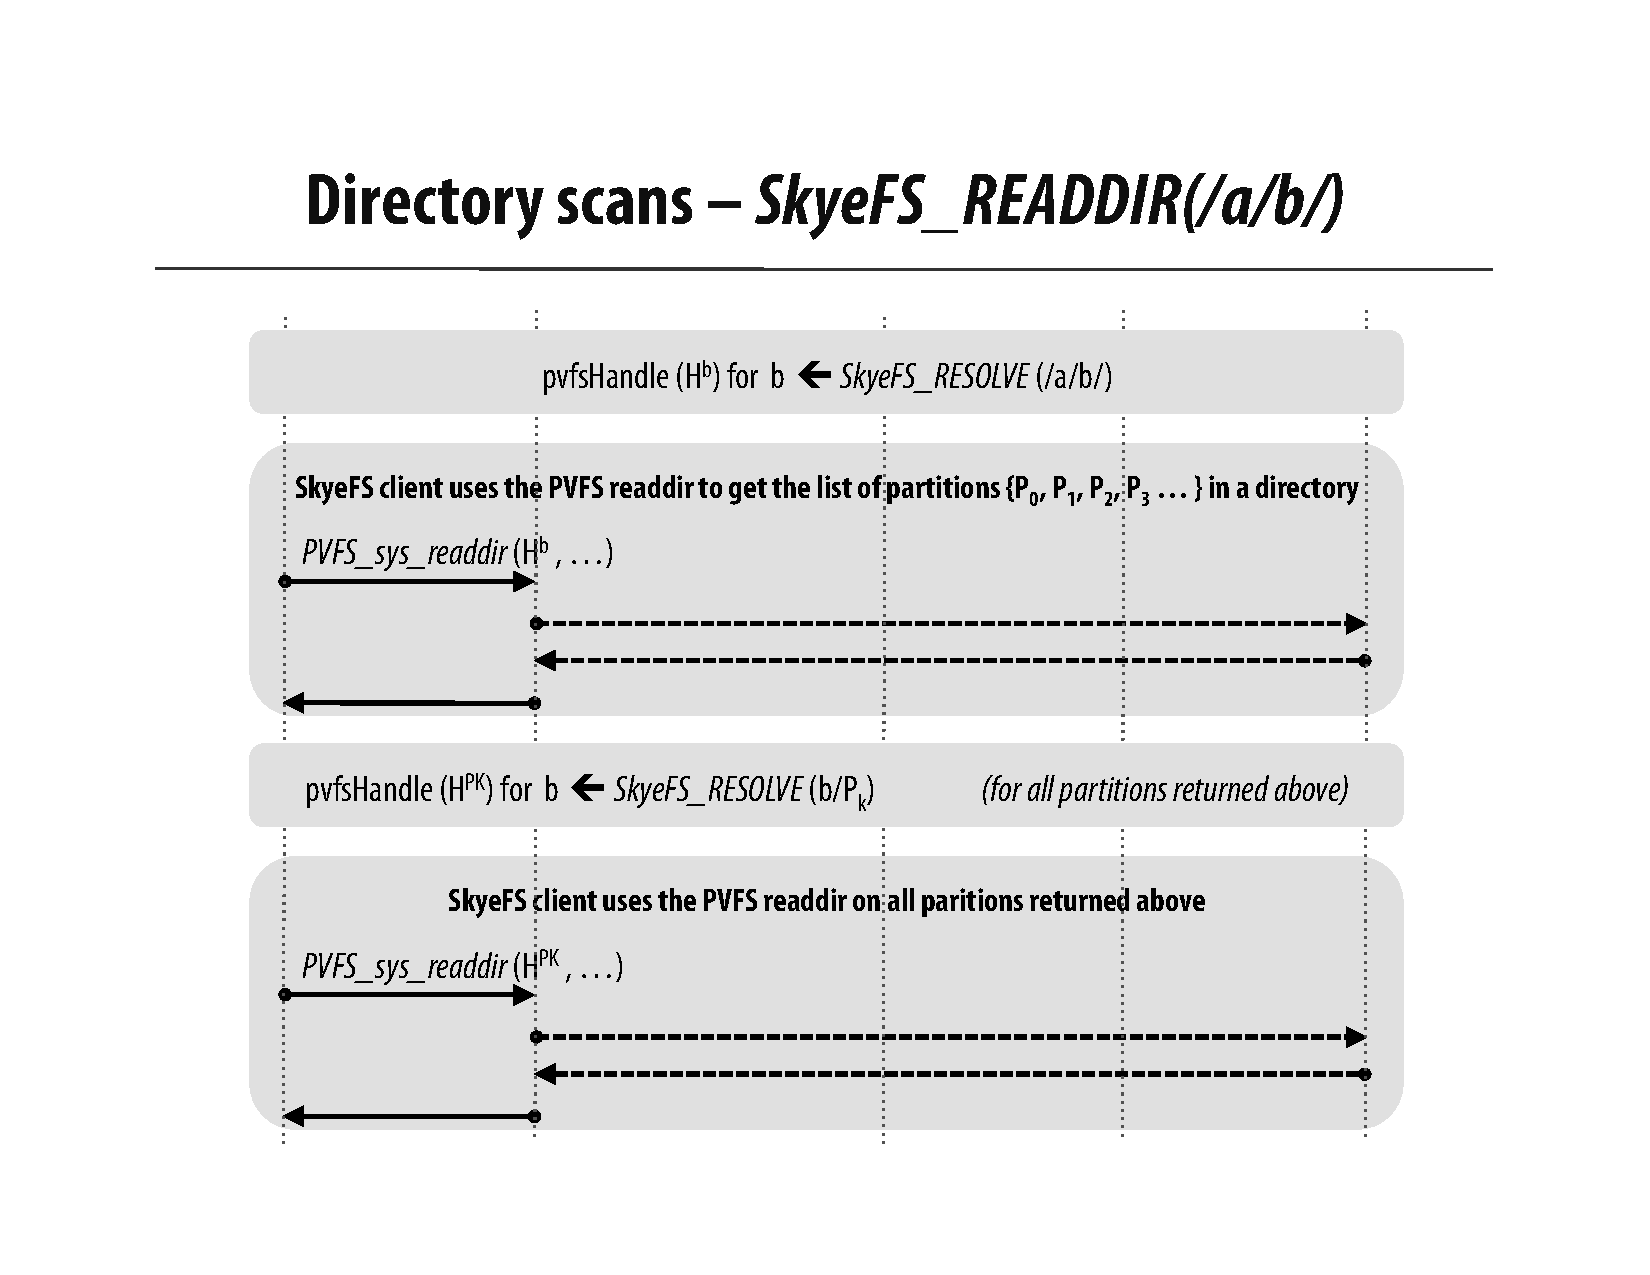
\includegraphics[scale=0.4]{figure-readdir}
\end{center}
\caption{SkyeFS readdir()}
\end{figure}
The readdir() operation requires some modification to handle the Giga+
partitioning.  While PVFS provides directory versioning to allow clients to
get a consistent snapshot of a directory we do not provide any such mechanism
to our users.  Instead, our readdir() mechanism is a ``best effort'' attempt
at providing a listing of the directory.  To accomplish this the client will
perform a PVFS\_sys\_readdir() of the logical directory handle returned by
lookup().  The client will then perform a PVFS\_sys\_readdir() of all handles
returned aggregating the results.  This naive approach will enter both real
partitions and splitting partitions.  While this may result in some files
being returned twice or not at all it is an inexpensive approach that will
work well in static or small directories.  We anticipate that the directories
for which this approach fails are too big for readdir() to be useful.

\subsection{Other Operations}
\begin{figure}
\begin{center}
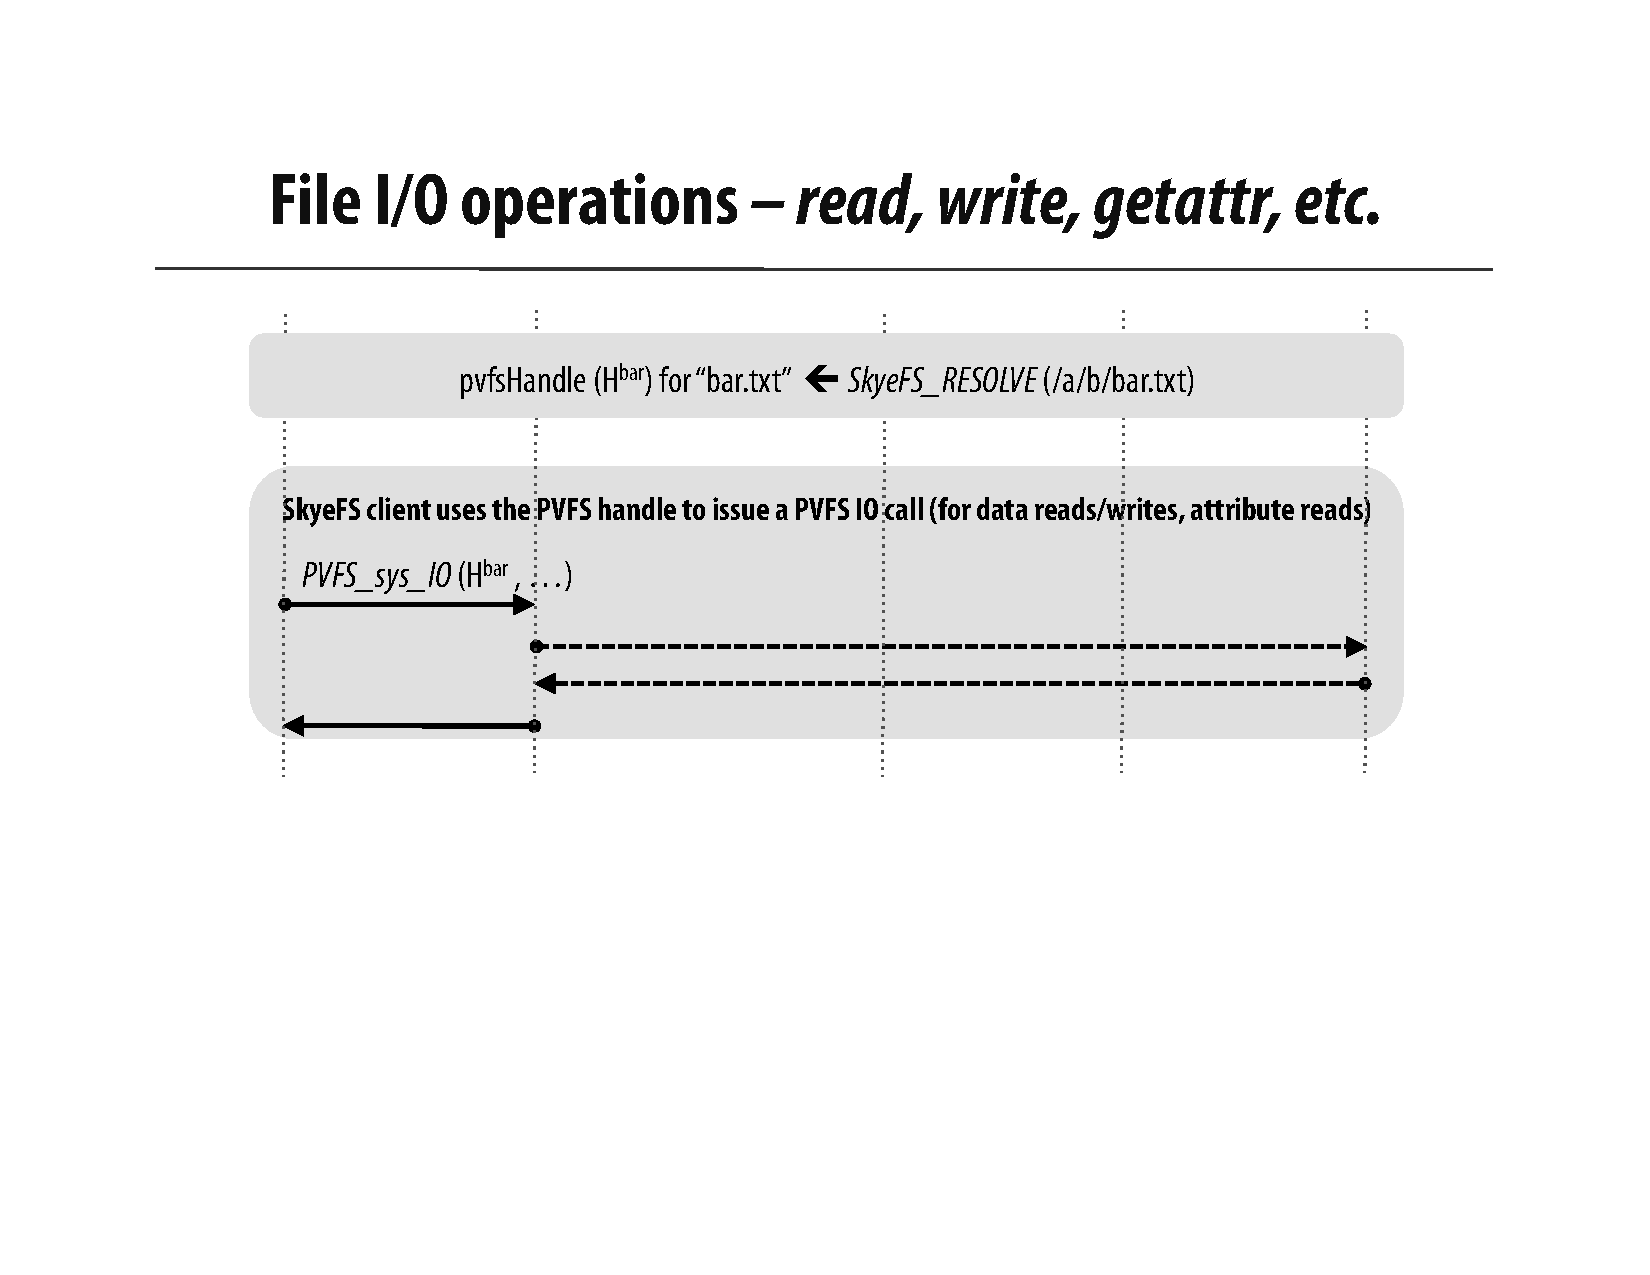
\includegraphics[scale=0.4]{figure-other}
\end{center}
\caption{SkyeFS IO Operations}
\end{figure}
All other operations are relatively straightforward modifications of their
pvfs2\-fuse counterparts with the PVFS lookup() operation replaced by our own
version.  This includes both data operations such as read() and write() as well
as metadata operations like stat() and chmod().  Because we resolve all objects
to stable PVFS handles inside their Giga+ partitions, these operations can
proceed on the client without concern for future splitting.

\section{Other Considerations}
\subsection{Multi-step Lookup}
In the current system, a lookup() call can only descend one step in a path
traversal.  Future work could extend the operation to provide the entire path
tho the \code{skye\_\-server} and allow the server to descend as many directories in the
path as it owns.  This would be of limited value in the current system where the
servers for a parent and child directory are chosen independently.  At the cost
of load balancing, parent and child directories could be placed on the same
server more often than chance to allow this mechanism to speed directory lookups
in more cases.  One example scheme to achieve this would be to place all new
directories on the same server as their parent.  When a directory splits the
first time the zeroth server would be moved to a new server chosen at random.
This would have the effect of keeping strings of small (and likely low-traffic)
directories on the same server while still ensuring that large directories are
load-balanced.

\subsection{Server Addition}
PVFS includes very limited support for server addition.  While new servers can
be added to the configuration file for a filesystem and brought online they must
take a previously unoccupied part of the handle space and there exists no
mechanism for automatically migrating either data or metadata to the new server.
The current SkyeFS implementation includes no specific provisions for addition
of servers, however future work could use SkyeFS to support the migration of
some data to new PVFS MDS.  In particular, by splitting overfull but already
load-balanced directories to these new servers some load can be moved to the
servers in already existing directories.  Because SkyeFS stores the number of
servers existing at the time of creation in each directory as an extended
attribute of that directory,\footnote{This is currently unimplemented.} no
specific mechanism is needed to add a new server other than adding the server
to the PVFS cluster and restarting all \code{skye\_\-server} processes.  However,
this mechanism is untested.

\subsection{Fault Tolerance}
PVFS is not a redundant file system and so it has very limited support for fault
tolerant or highly available configurations.  As a result, we do not make any
attempts to provide redundant services or fall over support in the case of
failures.  We assume that \code{skye\_\-server} processes and the PVFS servers fail
together and that any failure will render the system unusable until resolved by
restarting the system.

However, we do make every effort to leave the system in a usable state at all
times should any component fail.  Any skye process can fail at any time and the
resulting state will be repaired transparently upon restart.  This is primarily
due to the lack of additional SkyeFS metadata that is required on top of the
PVFS file system.  By carefully controlling the sequence of actions we take on
the PVFS file system we are able to ensure that any state of PVFS is
recognizable as either complete or the result of an unfinished action which can
then be resumed or aborted.

\subsection{Client and Server Thread Models}
Our current threading model for the \code{skye\_\-server} is based on the initial Giga+
prototype system in which a new thread is spawned for each connecting client.
When large numbers of clients are active this has the potential to be a
performance issue.  Other architectures for the server should be considered. 

On the \code{skye\_\-client} side we currently single thread the FUSE process causing all
operations to be serialized.  This is necessary because our initial tests
showed that the PVFS has the potential to stall when many requests using the
synchronous operations are in flight.  The recommendation from PVFS developers is
to switch to the low level FUSE interface and the asynchronous version of PVFS
operations.


\section{Conclusion and Take Aways}
We've described the design and implementation of the SkyeFS system.  The
following key design decisions were crucial to the success of the design.

\begin{itemize}
\item Minimization of work on the server by passing file handles back to the client
for non-conflicting operations
\item Avoidance of cross-RPC locks by either optimistic with retry strategies (in
the case of rename) or splitting operations into smaller atomic pieces (in the
case of remove).
\item Prevention of inconsistency issues by limiting amount of additional metadata
stored.
\end{itemize}

\end{document}
